\documentclass{article}

\author{Cronqvist, Fredrik \and Larsson, Sebastian \and Stenberg, Victor \and S\"{a}ll, Martin}
\date{\today}
\title{League of Legends learning analysis}

\usepackage{graphicx}

\begin{document}
\maketitle

\section{Introduction}
This report takes on the questions about where different level of experienced players have their fokus, priorities and if experience make it so the player can finish a game earlier. 

\subsection{League of Legends}
League of Legends (LoL) is multiplayer online battle arena (moba) game, two teams of five players with the goal to destroy the enemies base, called the Nexus. The player controls a hero on the battlefield trying to achive this goal. 

\section{Hypothesis and questions}
There is a distinct difference between how new players and experienced players look at the screen to attain information.
\begin{itemize}
\item Does the new players find the shop?
\item Do new players lay less time on the minimap then experienced players?
\item Are we able to improve the learningkurv for new players and still keep the enjoyment for the experienced players?
\item Are new players avalible to find the shop? %%behövs rättstavas
\end{itemize}

\section{Individual inspection}

\section{Grouped inspection}

\section{Conclusion}

\section{Discussion}

\section{Thank yous}

\begin{figure}[ht]
\begin{minipage}[b]{0.45\linewidth}
\centering
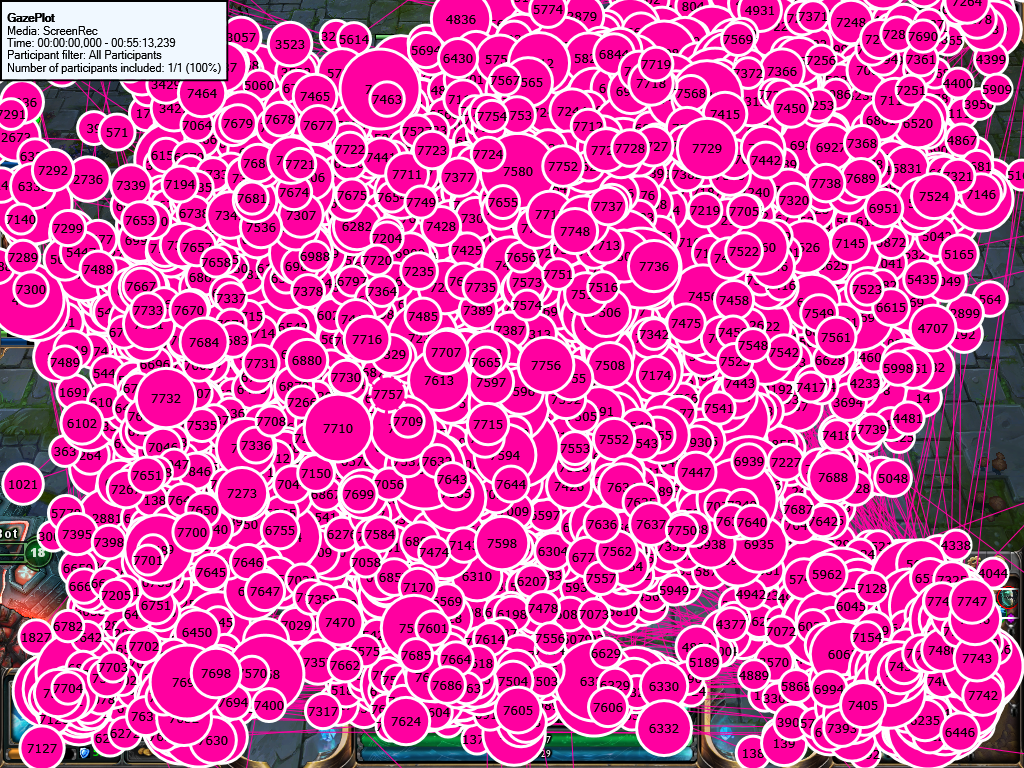
\includegraphics[width=\textwidth]{images/gazeplot/Emelie}
\caption{Gaze plot P1}
\label{gaze_eme}
\end{minipage}
\hspace{0.5cm}
\begin{minipage}[b]{0.45\linewidth}
\centering
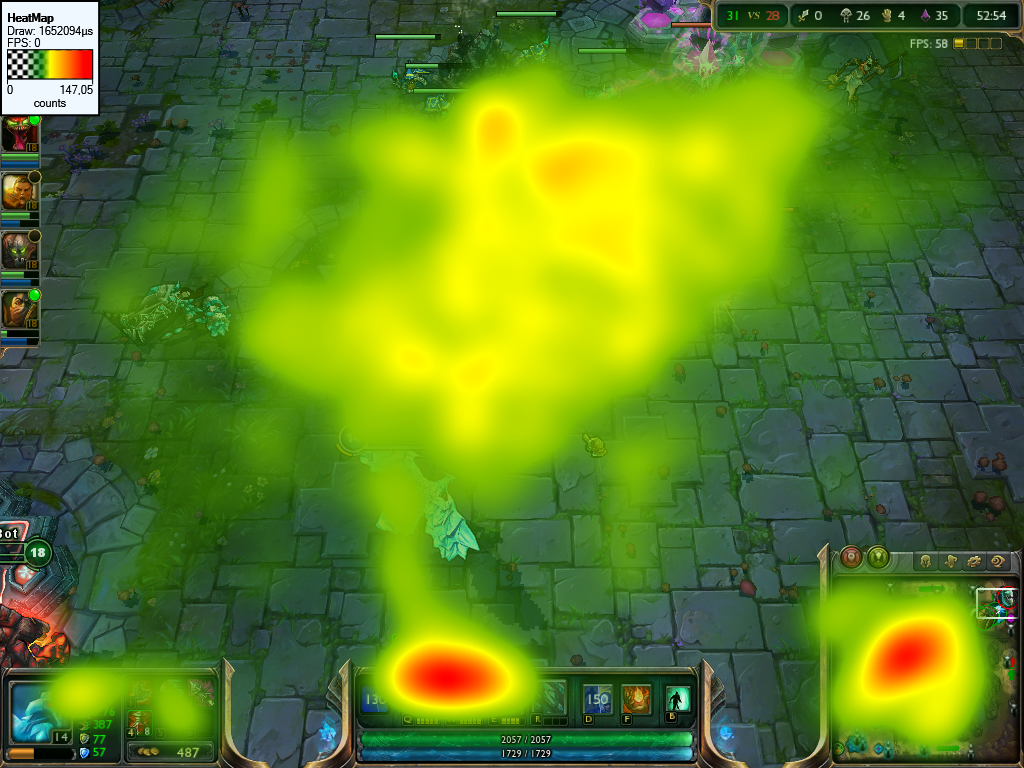
\includegraphics[width=\textwidth]{images/heatmap/Emelie}
\caption{Heat map P1}
\label{heat_eme}
\end{minipage}
\end{figure}

\begin{figure}[ht]
\begin{minipage}[b]{0.45\linewidth}
\centering
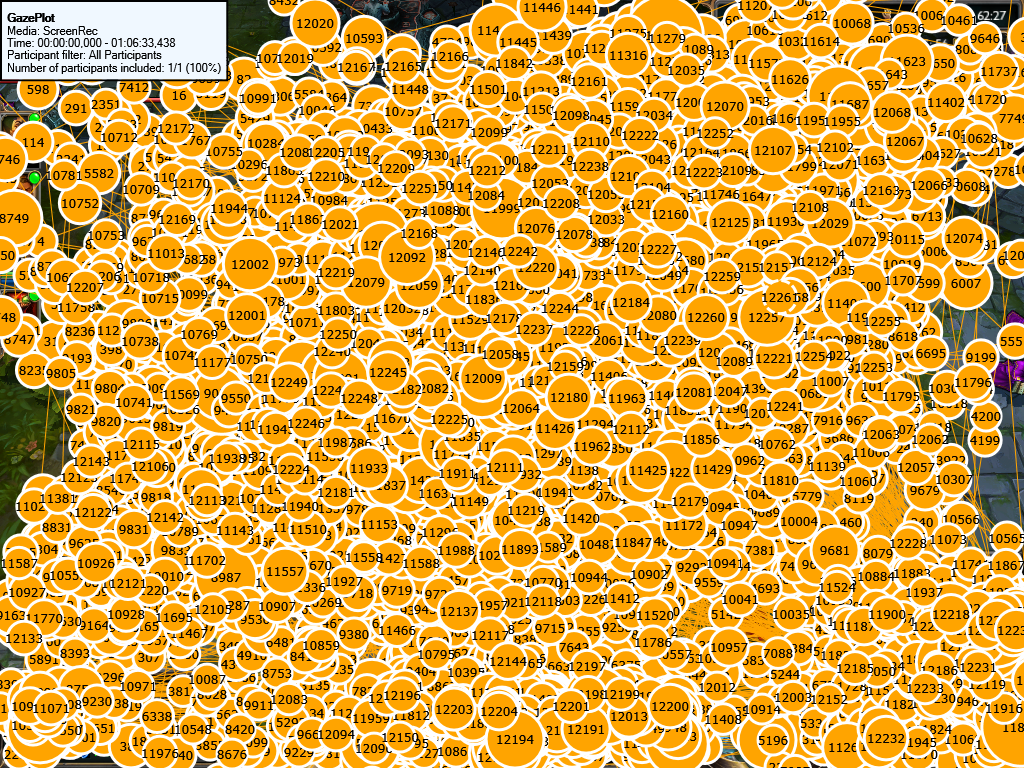
\includegraphics[width=\textwidth]{images/gazeplot/Pontus}
\caption{Gaze plot P2}
\label{gaze_pon}
\end{minipage}
\hspace{0.5cm}
\begin{minipage}[b]{0.45\linewidth}
\centering
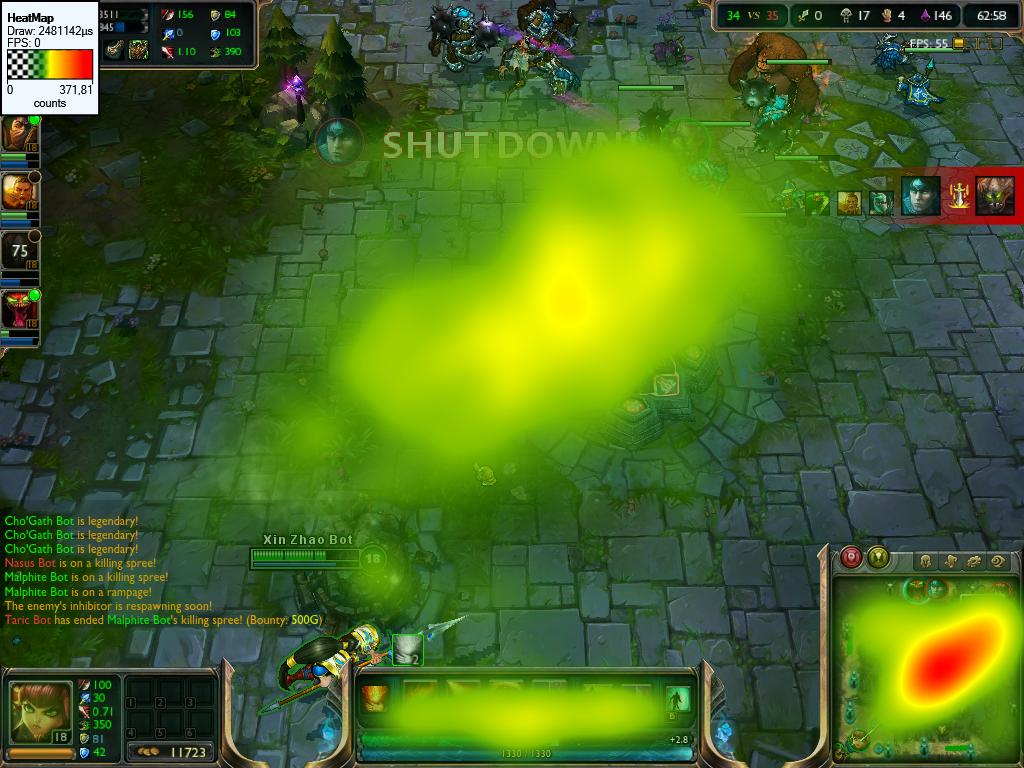
\includegraphics[width=\textwidth]{images/heatmap/Pontus}
\caption{Heat map P2}
\label{heat_pon}
\end{minipage}
\end{figure}

\begin{figure}[ht]
\begin{minipage}[b]{0.45\linewidth}
\centering
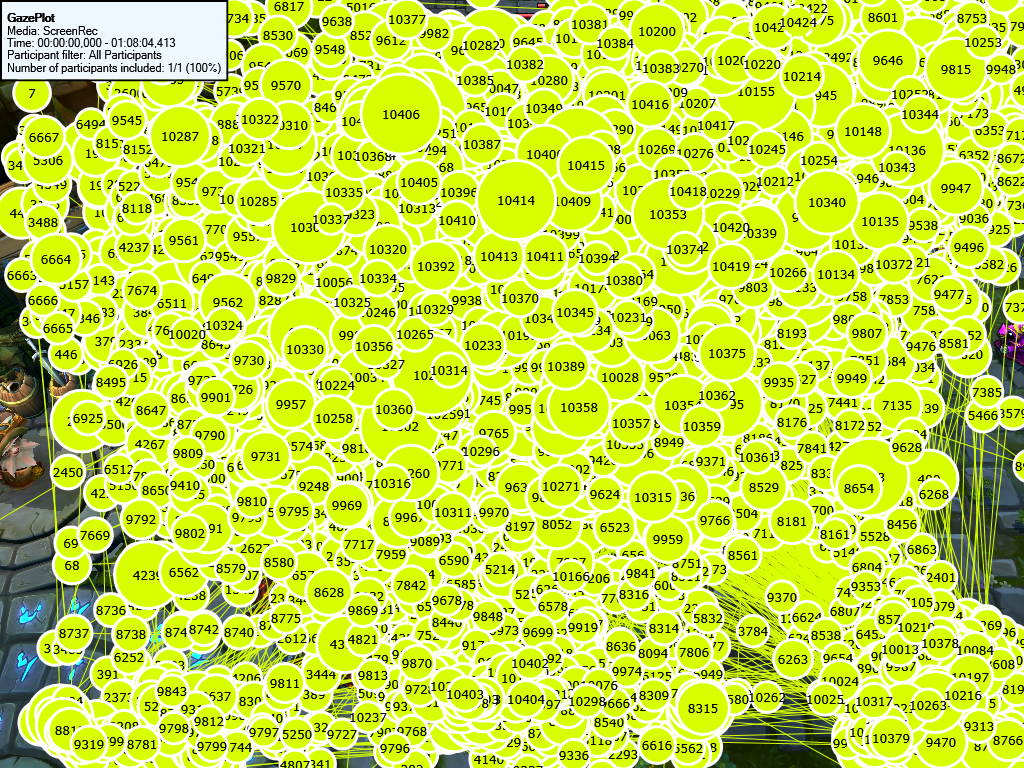
\includegraphics[width=\textwidth]{images/gazeplot/Sebastian}
\caption{Gaze plot P3}
\label{gaze_seb}
\end{minipage}
\hspace{0.5cm}
\begin{minipage}[b]{0.45\linewidth}
\centering
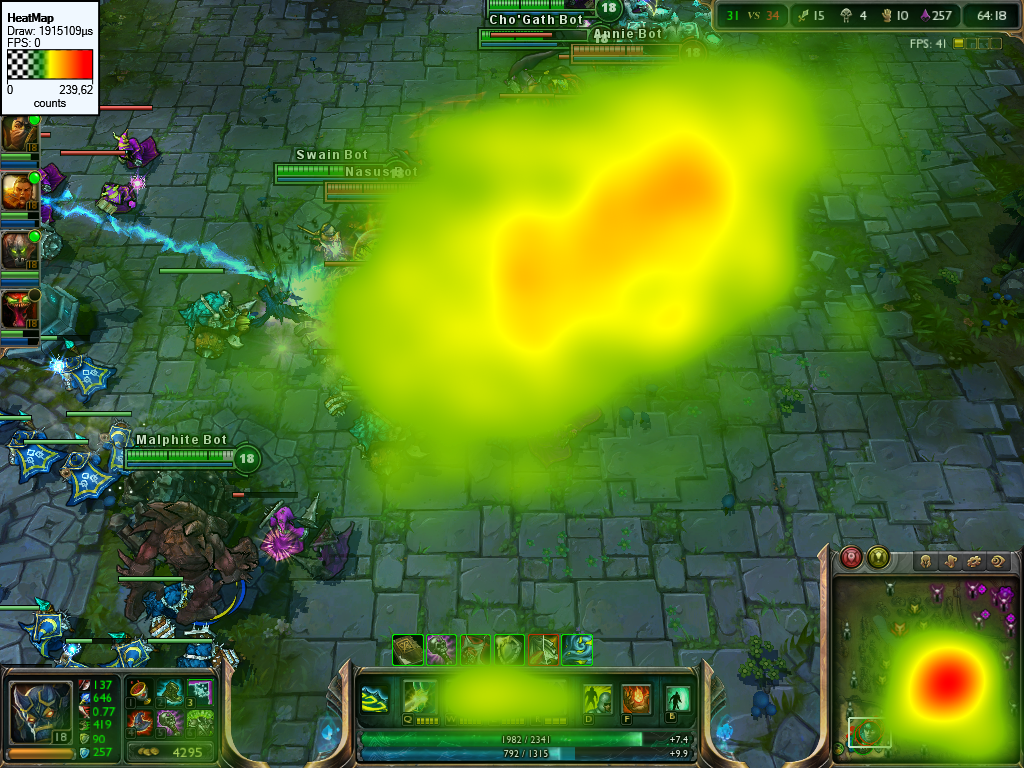
\includegraphics[width=\textwidth]{images/heatmap/Sebastian}
\caption{Heat map P3}
\label{heat_seb}
\end{minipage}
\end{figure}

\begin{figure}[ht]
\begin{minipage}[b]{0.45\linewidth}
\centering
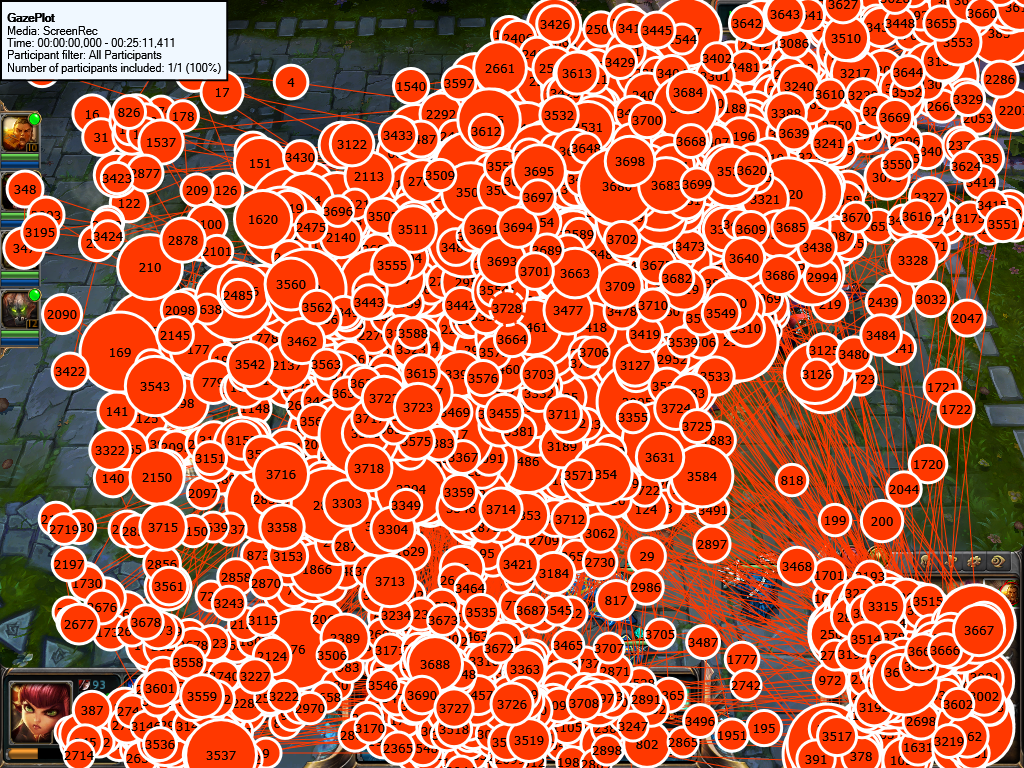
\includegraphics[width=\textwidth]{images/gazeplot/Victor}
\caption{Gaze plot P4}
\label{gaze_vic}
\end{minipage}
\hspace{0.5cm}
\begin{minipage}[b]{0.45\linewidth}
\centering
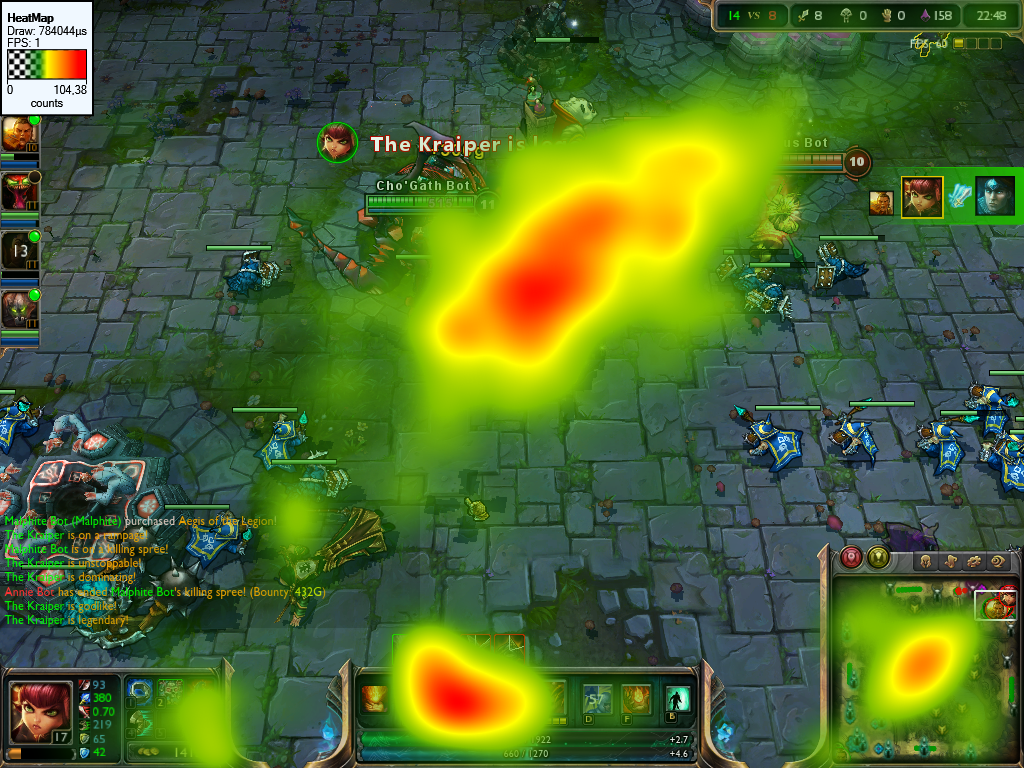
\includegraphics[width=\textwidth]{images/heatmap/Victor}
\caption{Heat map P4}
\label{heat_vic}
\end{minipage}
\end{figure}

\begin{figure}[ht]
\begin{minipage}[b]{0.45\linewidth}
\centering
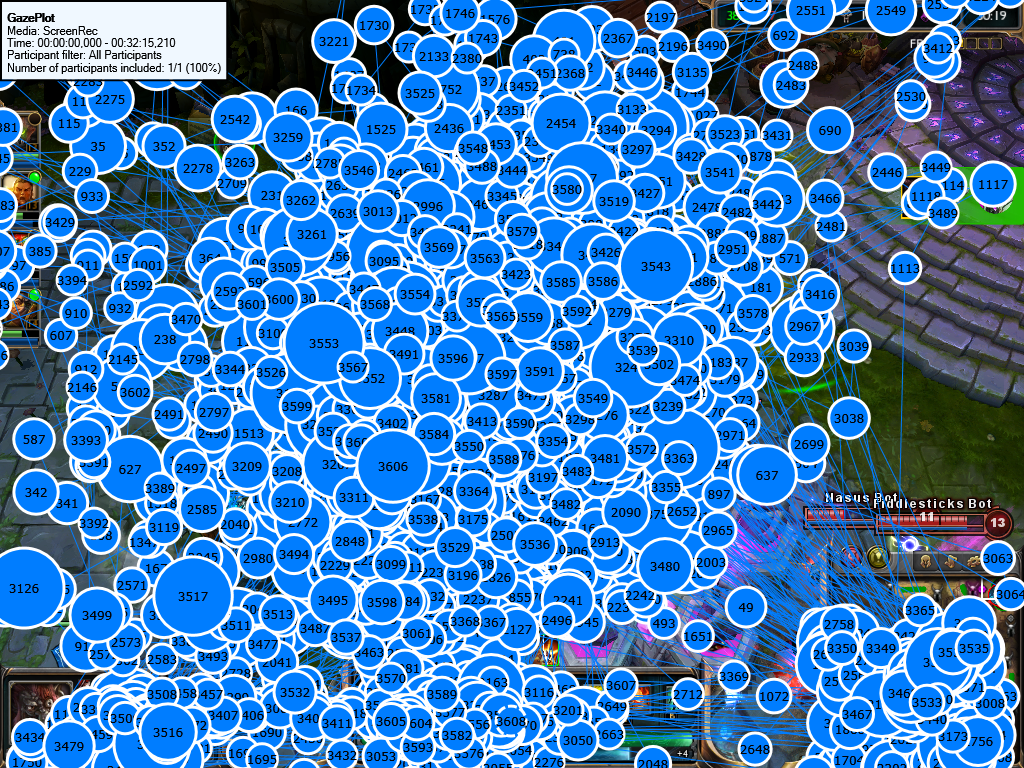
\includegraphics[width=\textwidth]{images/gazeplot/Fredrik}
\caption{Gaze plot P5}
\label{gaze_fre}
\end{minipage}
\hspace{0.5cm}
\begin{minipage}[b]{0.45\linewidth}
\centering
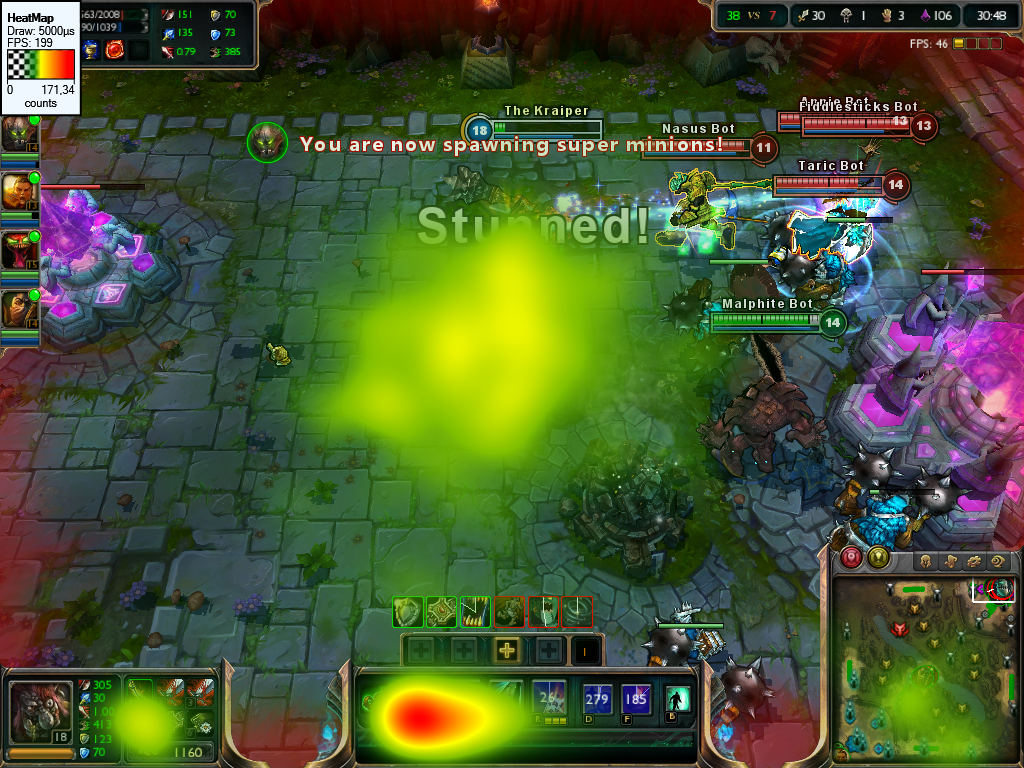
\includegraphics[width=\textwidth]{images/heatmap/Fredrik}
\caption{Heat map P5}
\label{heat_fre}
\end{minipage}
\end{figure}

\begin{figure}[ht]
\begin{minipage}[b]{0.45\linewidth}
\centering
\includegraphics[width=\textwidth]{images/gazeplot/Martin}
\caption{Gaze plot P6}
\label{gaze_mar}
\end{minipage}
\hspace{0.5cm}
\begin{minipage}[b]{0.45\linewidth}
\centering
\includegraphics[width=\textwidth]{images/heatmap/Martin}
\caption{Heat map P6}
\label{heat_mar}
\end{minipage}
\end{figure}

\end{document}
